\hypersetup{bookmarksopen=false}

\part{运动}
\markboth{运动}{运动}

\chapter{第一步} \label{chap:chap1}

当时已是凌晨一点钟;雨点凄厉地拍打着窗玻璃,我的蜡烛快要燃尽了。
这时,借着半熄灭的微光,我看到那怪物睁着一只暗黄色的眼睛;它呼吸急促,四肢抽搐着。

\begin{flushright}
	——玛丽$\cdot$雪莱,《弗兰肯斯坦》(1818)\\
\end{flushright}


\begin{figure}[!htb]
	\centering
	\includegraphics[width=0.5\linewidth]{chap1/1_0}
	% 加星号(*)表示不加编号
	\caption*{ \label{fig:1_0}}
\end{figure}

当玛丽$\cdot$雪莱写下那本让她名声大噪的哥特式小说时,全世界仍在为电的发现而兴奋不已——而路易吉$\cdot$加尔瓦尼的惊人发现——电刺激竟能使死青蛙的肌肉抽搐。
雪莱几乎可以想象,电流能使一个完整的生命体复活。


如今,距离伽伐尼的演示已过去两个世纪,肌肉电刺激技术对生活产生了深远的积极影响。
每个机场、学校和医院都安装了电除颤器,它们已经让成千上万的人的心脏重新跳动,而如果没有对心肌进行强力电击,这些人可能会死亡。
一项名为功能性电刺激的更先进技术已被开发出来,它可以使各种瘫痪患者的肌肉恢复活力,从而改善他们的生活质量。


在功能性电刺激中,电极要么贴在皮肤上,要么植入瘫痪肌肉中,靠近支配这些肌肉的神经。
电脉冲通过电极传输到神经,进而引起相关肌肉收缩并产生力量。
肌肉电刺激使瘫痪患者在躯干和腿部肌肉得到适当激活和协调的情况下能够站立和行走。
2016 年,几名脊髓损伤导致胸部以下瘫痪的患者参加了一项名为“Cybathlon”的全新国际自行车比赛。
获胜者在不到 3 分钟的时间内骑行了 750 米。


功能性电刺激远不止向神经和肌肉输送电流那么简单。
对于健全人来说,神经系统协调着许多肌肉,使我们能够行走、跑步或骑自行车,就像指挥家协调管弦乐队的乐手一样。
当 Cybathlon 比赛的冠军在赛道上骑行时,能够传送多达 24 个通道的精确定时刺激,以协调他原本瘫痪的肌肉产生的力量。
即使达到了这种复杂程度,结果也并非完美。
关于我们的肌肉如何协同工作以创作运动之乐,我们仍有许多需要学习的地方。


在本书中,我们将探索这首宏伟的交响曲。
我们将从力学的视角审视人类和动物的运动,以理解运动的生物力学。
我们将运用简单的概念模型来解答诸如为何行走和跑步是高效的运动方式、为何宇航员在月球上采取跳跃式步态,以及跑道和跑鞋如何提升运动表现并减少损伤等问题。
我们将深入研究肌肉的结构,直至其微观的动力产生机制,并精确观察电刺激如何促使肌肉收缩。
我们将描述用于生成运动模拟的复杂计算工具,从而使我们能够估算产生这种运动的肌肉力量。
这些模拟向我们展示了我们在行走、跑步或骑自行车时如何协调肌肉。
事实上,肌肉驱动的模拟对于 Cybathlon 金牌团队来说是一个宝贵的工具。


本书始终强调既定理论,为理解运动生物力学奠定基础,并涵盖计算机模拟、移动运动监测和可穿戴机器人等领域基于这些基础的创新。
许多近期的进展都由科幻小说所预见,并为我们展现未来新技术的雏形。
其中一些愿景或许如同唤醒弗兰肯斯坦的怪物般奇幻,而另一些则近在眼前。
无论如何,我们都在探索这个激动人心领域的潜力。






\section{我们为什么研究运动}

运动令人着迷,是生命的基础。
我们的身体功能多样,既能展现力量,又能展现灵巧。
运动对于维持身心健康至关重要。规律的体育锻炼有助于预防心脏病、癌症、骨质疏松症、肥胖症、糖尿病、抑郁症、焦虑症和其他严重疾病,然而,全球只有不到一半的人口能够充分活动以维持身心健康。
体育锻炼是一剂强效且廉价的良药,即使少量运动也能带来显著的健康益处。
在研究运动生物力学的过程中,我们致力于理解运动产生的生物结构和过程,并将这些知识应用于提高灵活性、体育锻炼能力和健康水平。


运动生物力学领域历史悠久。
如同人类的许多追求一样,推动其进步的动力源于改善生活的渴望,以及对环境和自身与生俱来的好奇心。
亚里士多德在公元前350年左右撰写了第一本探讨动物运动一般原理的著作,书名恰如其分地命名为《动物运动论》。
他和其他古希腊人认为,当肌肉被“气”(pneuma)(流经我们神经的“生命之气”)充气时,肌肉就会收缩。


此后,无数学者推动了该领域的发展,本书将介绍其中一些学者。
生物力学的先驱包括列奥纳多$\cdot$达$\cdot$芬奇(1452-1519),他绘制了数百幅详细的解剖图,并研究了肌肉骨骼系统的力学功能(图~\ref{fig:1_1})。
乔瓦尼$\cdot$博雷利(1608-1679)是第一个运用力学定律将肌肉施加的力与其在关节周围产生的力矩联系起来的人(图~\ref{fig:1_2})。
然而,博雷利仍然坚持经典观点,认为肌肉是通过气动、膨胀过程收缩的。
这一理论遭到了佛罗伦萨宫廷中博雷利的对手尼古拉斯$\cdot$斯坦诺(Nicolas Steno,1638-1686)的反驳,他指出肌肉在收缩时体积保持不变——我们将在第 4 章中研究这个悖论。
后来,路易吉$\cdot$加尔瓦尼(Luigi Galvani,1737-1798)发现了电信号能够引起肌肉收缩这一此前未被怀疑的能力,从根本上奠定了我们现代电生理学领域的基础。
最后,我不能不提一下埃德沃德$\cdot$迈布里奇(Eadweard Muybridge,1830-1904),他在距离我家约一公里(现在的斯坦福大学校园)的地方进行了早期的人类和动物运动摄影研究。迈布里奇的照片即使在今天看起来也令人着迷,它们是电影和生物力学史上的里程碑(图~\ref{fig:1_3})。
事实上,电影制作技术和生物力学科学仍在齐头并进。


\begin{figure}[!htb]
	\centering
	\includegraphics[width=0.75\linewidth]{chap1/1_1}
	\caption{列奥纳多$\cdot$达$\cdot$芬奇笔记本中的一页,展示了他的肌肉力线概念。
		图片由皇家收藏信托基金会提供。 \label{fig:1_1}}
\end{figure}


\begin{figure}[!htb]
	\centering
	\includegraphics[width=0.75\linewidth]{chap1/1_2}
	\caption{乔瓦尼$\cdot$博雷利(Giovanni Borelli)对人体肌肉和关节的静态分析,他常被誉为生物力学之父。
		图片来自《动物运动》(De motu animalium)。 \label{fig:1_2}}
\end{figure}


\begin{figure}[!htb]
	\centering
	\includegraphics[width=1.0\linewidth]{chap1/1_3}
	\caption{动作捕捉先驱埃德沃德$\cdot$迈布里奇的一系列照片。
		图片由斯坦福大学提供。  \label{fig:1_3}}
\end{figure}


如今,生物力学是一个快速发展的多学科领域,汇聚了众多科学和工程领域的专家学者的通力合作。
生物学家利用生物力学的洞见来理解动物形态与功能之间的关系:
例如,蜥蜴如何跳跃并抓住墙壁(图~\ref{fig:1_4}),或者霸王龙是否能够奔跑(第~\ref{chap:chap3}~章)。
神经科学家研究大脑如何在运动过程中协调肌肉,以及这些神经回路在受伤和患病的情况下如何受到干扰。
外科医生可以使用生物力学模型来确定脑瘫患者是否能从肌腱延长手术中受益。
机器人专家正在发明日益精密的假肢(图~\ref{fig:1_5})和能够在危险环境中执行复杂任务的双足机器人。
运动科学家分析运动动作,例如“背越式跳高”(第~\ref{chap:chap9}~章),以了解如何提高运动表现并预防伤病。
计算机科学家和生物力学工程师开发新的算法和软件工具来模拟运动并从这些模拟中获得见解。


\begin{figure}[!htb]
	\centering
	\includegraphics[width=1.0\linewidth]{chap1/1_4}
	\caption{红头鬣蜥在飞行过程中用尾巴控制身体方向。
		这只蜥蜴准备抓住右侧的垂直墙壁,它顺时针旋转尾巴,通过角动量守恒使身体保持垂直。
		图片由罗伯特$\cdot$富尔提供。 \label{fig:1_4}}
\end{figure}


\begin{figure}[!htb]
	\centering
	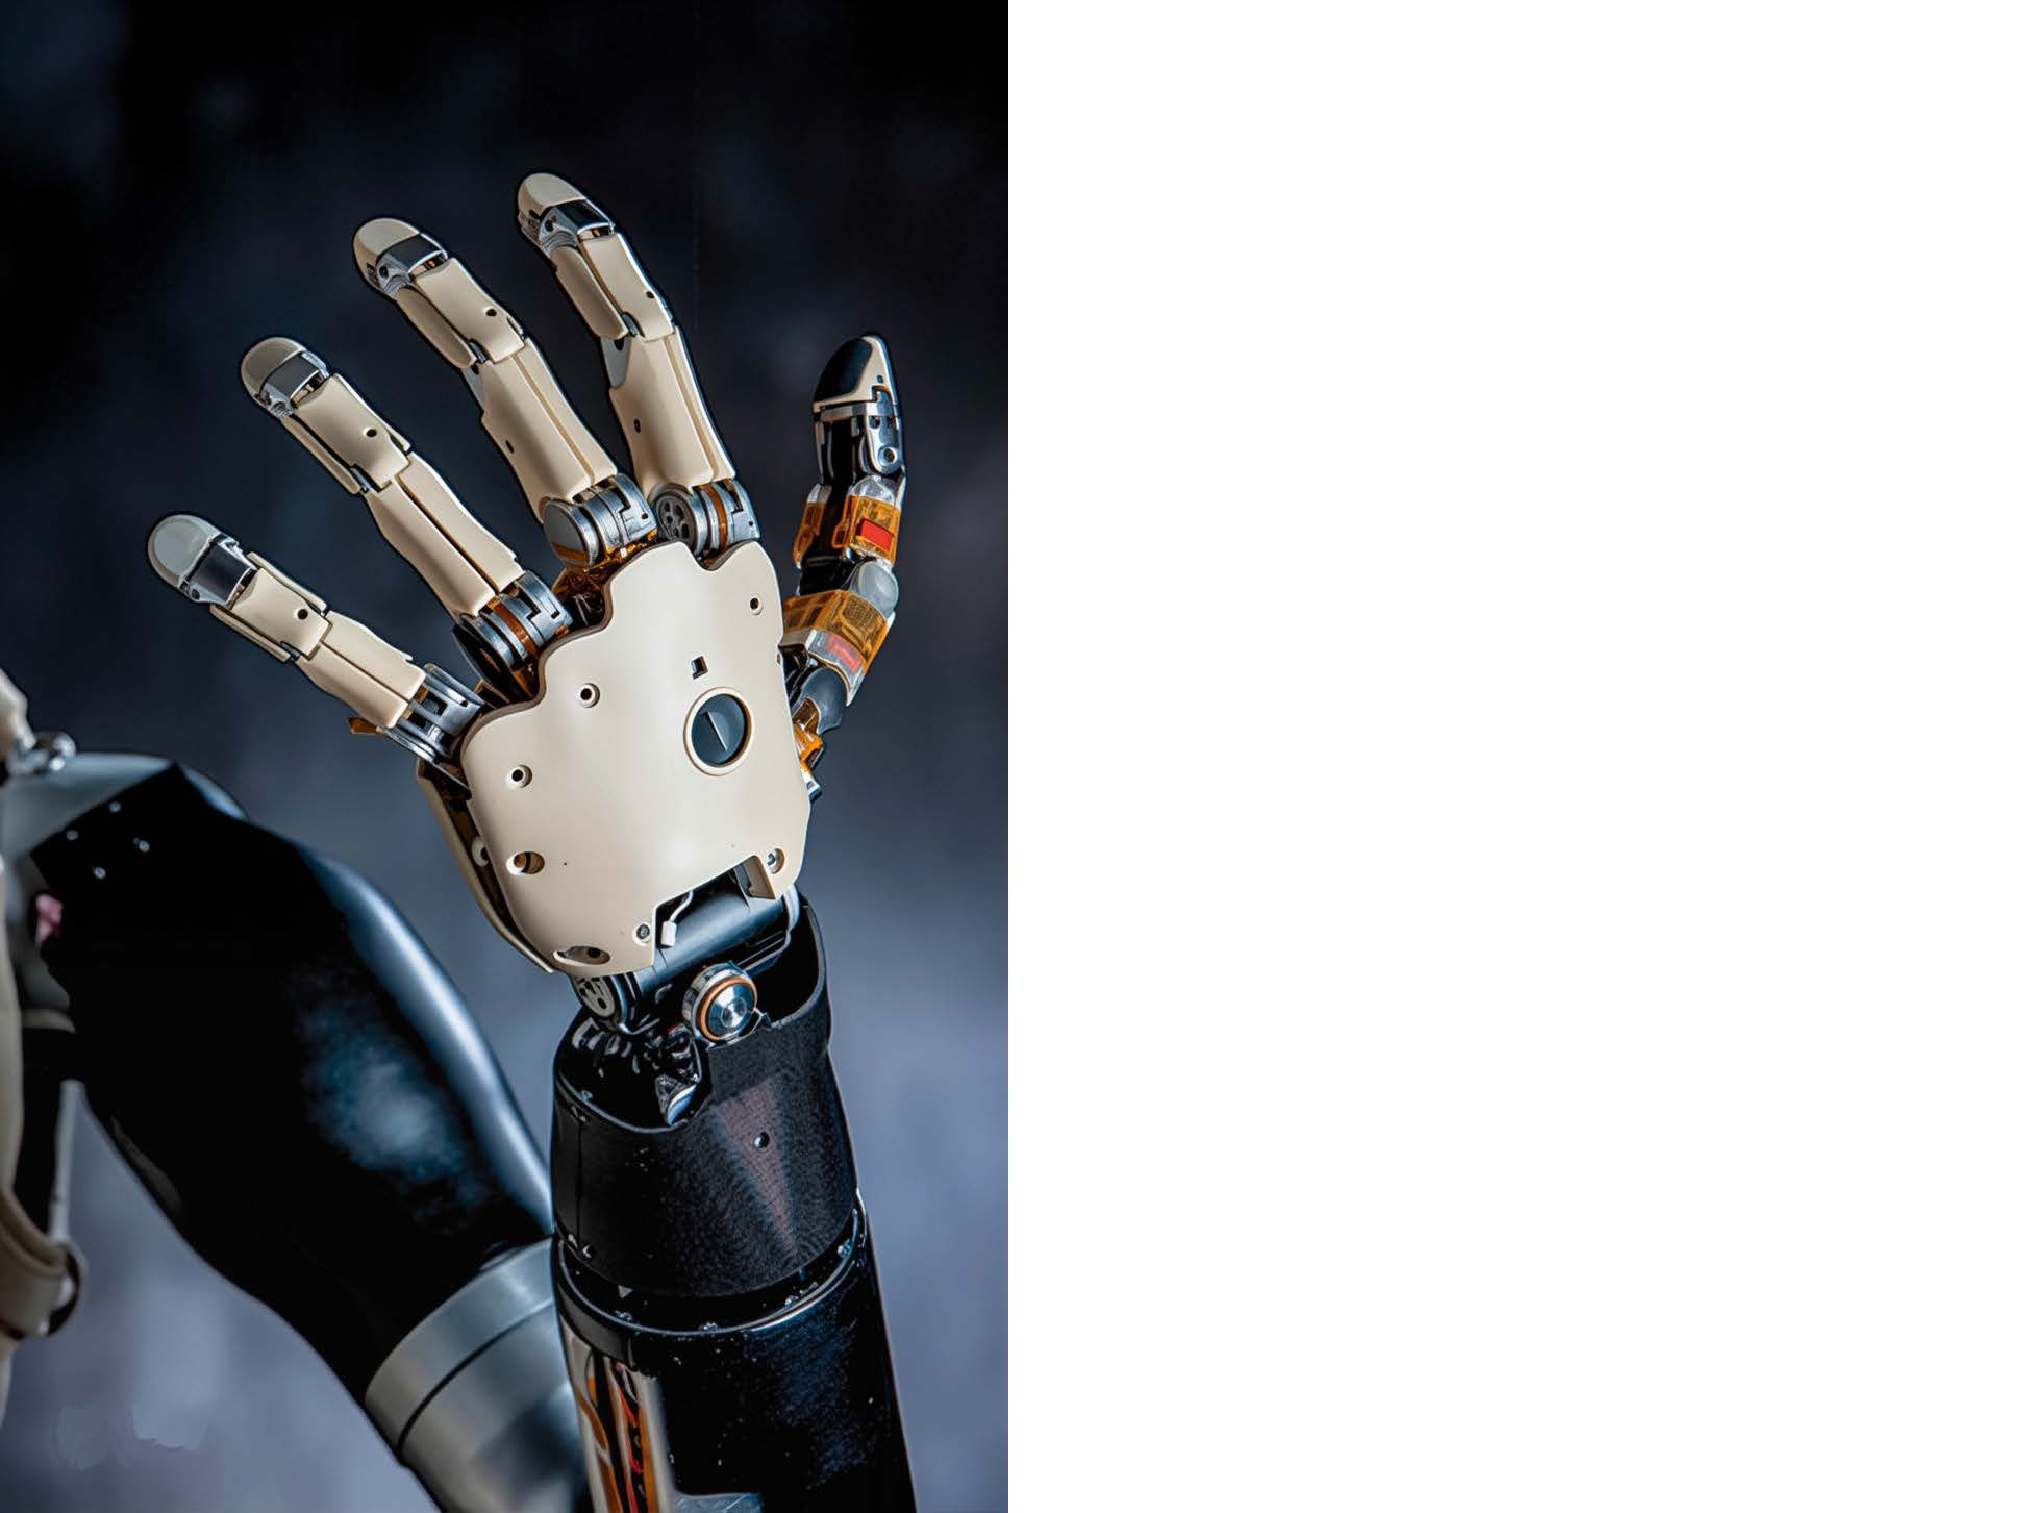
\includegraphics[width=0.5\linewidth]{chap1/1_5}
	\caption{功能强大的假肢如今触手可及。
		图片由约翰$\cdot$霍普金斯大学提供。 \label{fig:1_5}}
\end{figure}


生物力学甚至在科学领域之外也发挥着作用。电影制作人运用生物力学和动作捕捉技术,为游戏和电影创作计算机生成的图像,风格各异,从奇幻到逼真(图~\ref{fig:1_6})。
其成果将美感与科学的准确性完美结合,这在一两代人之前是难以想象的。


\begin{figure}[!htb]
	\centering
	\includegraphics[width=1.0\linewidth]{chap1/1_6}
	\caption{图片来自电影《阿凡达》和行为艺术家詹$\cdot$斯塔福德。
		她的动作被动作捕捉技术记录下来,并制作成计算机生成的图像。
		图片由二十世纪福克斯公司提供。 \label{fig:1_6}}
\end{figure}


总的来说,这些努力极大地改善了我们的生活。
现在,我们可以根据保持健康所需的日常体力活动水平获得建议,并且我们可以使用有助于我们实现健身目标的工具。
装配线、办公家具和许多消费品都符合人体工程学设计,以提高舒适度并防止受伤。
一些产品和程序已被设计用于置换髋关节和膝关节,减轻疼痛并恢复数百万骨关节炎患者的功能。
动力外骨骼正在彻底改变中风后康复,并可以使瘫痪患者恢复运动能力。
帕金森病等运动障碍已通过深部脑刺激得到成功治疗,深部脑刺激是指植入电极向大脑特定区域传递电脉冲。
硬膜外刺激是一种激活脊髓神经回路的技术,最近已显示出帮助脊髓损伤患者恢复自主运动的潜力。
运动员正受益于旨在降低受伤风险并提高运动表现的设备和训练计划(图~\ref{fig:1_7})。


\begin{figure}[!htb]
	\centering
	\includegraphics[width=0.6\linewidth]{chap1/1_7}
	\caption{生物力学研究有助于打造能够最大限度提升运动表现的运动器材。
		这款冰鞋的靴子和冰刀之间的铰链设计延长了冰刀与冰面的接触时间,从而增加了推进力的持续时间,从而提高了速度。
		图片由 McSmit 提供。 \label{fig:1_7}}
\end{figure}



\section{半机械人奥运会}


或许,更深入地观察一个引人注目的例子——“Cybathlon”(人机合体竞技),就能更好地理解生物力学的影响。
2016年,苏黎世联邦理工学院(ETH Zurich)教授罗伯特$\cdot$里纳(Robert Riener)组织了首届“Cybathlon”,这是一项将科学与体育进行创新性融合的运动。
与残奥会不同,这项运动的比赛项目侧重于日常任务。
例如,佩戴假肢的运动员比赛搬运物品、切面包、开罐子和晾衣服。
佩戴假肢的运动员比赛爬坡和上楼梯,同时保持杯子在碟子上保持平衡。
为了强调这项比赛关乎人类与科技的结合,参赛者被称为“飞行员”,而不是“运动员”。


在这场非传统的比赛中,最传统的体育项目是腿部瘫痪者自行车赛。
金牌被凯斯西储大学在罗纳德$\cdot$特里奥洛(Ronald Triolo)的科研领导下夺得。
该队的车手是马克$ \cdot $穆恩(Mark Muhn)(图~\ref{fig:1_8}),他在2008年的一次滑雪事故中脊髓受伤,胸部以下瘫痪。


\begin{figure}[!htb]
	\centering
	\includegraphics[width=0.6\linewidth]{chap1/1_8}
	\caption{马克$\cdot$穆恩参加 Cybathlon 比赛。
		图片由 Paul 和 Gabrielle Marasco 提供。 \label{fig:1_8}}
\end{figure}


凯斯西储大学的团队在功能性电刺激领域研究了四十年,并开发出了首批植入式神经肌肉刺激器。
特里奥洛相信,他们在植入电极方面的经验将成为制胜优势,因为其他团队正在使用通过皮肤传输电信号的电极。
植入电极可以更精准地刺激被激活的肌肉,从而产生更强烈的肌肉收缩。


该团队通过多种方式最大限度地提高了获胜的几率(McDaniel 等人,2017)。
他们购买了一辆卧式自行车,并将其拆解,去掉了所有不必要的重量。
他们让飞行员(最初有五名,其中两名被选中前往苏黎世)参加了强化训练计划。
我们最感兴趣的是他们使用的生物力学模型(图~\ref{fig:1_9})。


\begin{figure}[!htb]
	\centering
	\includegraphics[width=1.0\linewidth]{chap1/1_9}
	\caption{用于调整肌肉兴奋模式以产生循环的肌肉驱动生物力学模型的示例。 \label{fig:1_9}}
\end{figure}


特里奥洛表示,这些模型与我们在本书后面描述的类似,在两个方面发挥了作用:
首先,它消除了“死胡同”(行不通的想法);
其次,它优化了提供给飞行员的电刺激模式。
每块腿部肌肉的每一次收缩都由一个外部控制装置(一个绑在飞行员腰间的盒子)控制。
为了安全起见,飞行员可以控制盒子的开关。


为了获得刺激模式,研究小组从文献中获取了自行车运动的生物力学模型,并根据每位骑手的特点进行了定制。
定制非常重要,因为瘫痪后肌肉的特性会发生变化,而可以通过刺激激活的肌肉数量很少,所以适用于健全骑手的激活模式可能不适用于脊髓损伤患者的刺激驱动踩踏。
Musa Audu 带头为每位骑手建模和定制刺激模式,并采用第~\ref{chap:chap10}~章中描述的技术来估计每块肌肉激活的时间和强度。
值得注意的是,刺激模式在比赛期间从未改变。
当骑手的肌肉疲劳时,他的腿会保持以相同的速率抽动,但它们无法用那么大的力气推动,所以骑手必须换挡才能保持自行车前进。


事实上,飞行员之所以会很快感到疲劳,是因为功能性电刺激并不像大脑发出的自然信号那样募集肌肉纤维。
我们将在第~\ref{chap:chap4}~章中回顾这一现象,但现在只需说明,大多数自然发生的运动都是通过首先募集“慢肌”纤维(相对较小且抗疲劳),然后是“快肌”纤维(产生较大力量但很快疲劳)产生的。
然而,电刺激以相反的顺序募集肌肉纤维。
由于这种“反向募集”,飞行员在开始训练时几乎无法让摩托车持续行驶超过一分钟。



但意想不到的事情发生了——相比于单调乏味的固定自行车,飞行员们更喜爱比赛用自行车带来的户外锻炼。
而且运动训练可以增强瘫痪的肌肉。在飞行员们积极进取的激励下,经过5个月的训练,他们能够坚持骑车参加3分钟的比赛。
特里奥洛表示,他希望在未来几年找到一种技术解决方案来解决招募逆转问题,但在2016年,只有一个解决方案:“让我们的飞行员尽情锻炼”。
而且,这个方案真的奏效了!
在苏黎世,穆恩以2分58秒的成绩完成了750米的比赛,并夺得了金牌。


Cybathlon 的经历改变了 Muhn 的人生,或许更令人惊讶的是,它改变了 Triolo 的研究。
Triolo 说,以前他们的康复方法是任务导向的。
他们专注于让志愿者站立、行走或进行日常生活活动,比如穿衣和做饭。
但当他们的参与者在户外骑自行车,并开始在锻炼的同时享受乐趣时,一切都改变了。
他们锻炼得更多,这对他们康复的各个方面都产生了巨大的回报,包括提升了他们的自尊心。
当一名骑手在公共道路上骑自行车时,另一个骑手追上他并说:“轮子真漂亮。”
这几乎是陌生人第一次将他视为一个拥有酷炫自行车的人,而不是一个残疾人。



\section{研究运动的工具}

我写这本书的目标之一是让你熟悉我的团队和其他人员开发的肌肉驱动生物力学模型。重要的是要意识到这些模型是基于实验数据的。让我们来看看我们收集的数据类型。



分析运动的一种常用技术是在研究实验室和诊所录制个体的视频。
许多此类记录都是通过红外摄像机获得的,这些摄像机可以追踪贴在皮肤上的标记物,类似于电影制作中使用的技术(图~\ref{fig:1_10})。
最近,不需要标记物的运动捕捉技术变得越来越流行。
基于视频的系统已经广泛应用,但这些系统的普及程度已被惯性测量单元 (IMU) 所取代,IMU 现已集成到智能手机、可穿戴活动监测器和服装中。
IMU 能够在自然环境中长时间收集运动数据(速度和加速度),这对于监测病情进展和制定治疗方案非常有价值。
低成本活动监测器中 IMU 的普及也使得对全球数百万个体进行大规模研究成为可能(图~\ref{fig:1_11})。


\begin{figure}[!htb]
	\centering
	\includegraphics[width=1.0\linewidth]{chap1/1_10}
	\caption{前手翻(时长 2.9 秒)期间,贴在皮肤上的标记物轨迹。
		受试者最初站立(最左侧),然后向前跳跃,双手撑地翻身(中间),双脚落地,然后跳了一跳恢复平衡(最右侧)。
		球体间距越大,表示标记物移动速度越快。
		数据来自 ACCAD (2018)。 \label{fig:1_10}}
\end{figure}


\begin{figure}[!htb]
	\centering
	\includegraphics[width=1.0\linewidth]{chap1/1_11}
	\caption{717,527 名受试者超过 6800 万天的智能手机活动数据揭示了 111 个国家/地区的体力活动差异。
		图片改编自 Althoff 等人(2017 年)的研究,这是全球规模最大的体力活动调查\cite{althoff2017large}。 \label{fig:1_11}}
\end{figure}


在实验室或诊所进行实验时,除了运动捕捉系统外,还可能涉及多种专用设备。
我们经常使用测力板来测量脚和地面之间的力。在步行和跑步研究中,使用跑步机很方便,因为受试者可以保持在运动捕捉系统能够精确测量的范围内。
一些跑步机还配备了测量地面反作用力的仪器。
肌电图用于测量各种肌肉活动的时间和强度。
我们可以监测跑步者的呼吸,测量消耗的氧气量和产生的二氧化碳量,以估算跑步所需的代谢能量。
磁共振成像和荧光透视成像等成像技术的普及使我们能够看到运动中的动物或人体内部,为可视化和测量运动提供了强有力的工具。


概念模型可以成为强大的分析工具,正如我们将在本书中看到的。
例如,第~\ref{chap:chap2}~章和第~\ref{chap:chap3}~章展示了一个简单的摆模型如何为我们合理地模拟行走,而一个质量弹簧模型如何为我们提供关于跑步的重要见解。
一个能够完成任务的简单模型几乎总是比一个更复杂的模型更受欢迎,后者提供了类似的实用性,但构建和理解起来更困难。
当然,并非所有复杂现象都能用简单的力学模型来表示。
正如我们将在第~\ref{chap:chap11}~章和第~\ref{chap:chap12}~章中看到的,肌肉驱动的模拟是强大的工具,可以填补第~\ref{chap:chap2}~章和第~\ref{chap:chap3}~章中简单模型所缺失的许多细节。


计算机模拟可以计算无法直接测量的量并预测假设场景中的运动,从而对实验进行补充。
模拟有助于理解例如难以通过实验研究的损伤。我们还可以估算导致观察到的运动的肌肉力量,以及关节负荷、肌腱应变和其他无法测量的量。
在正向动态模拟中,我们规定一块或多块肌肉的神经激活模式,然后预测肌肉骨骼模型的最终运动(图~\ref{fig:1_12})。
需要实验数据来开发和测试用于运动模拟的肌肉骨骼动力学数学模型,并评估模拟反映现实的程度。


\begin{figure}[!htb]
	\centering
	\includegraphics[width=1.0\linewidth]{chap1/1_12}
	\caption{典型的正向动态模拟的要素。
		运动源于神经、肌肉、骨骼和感觉系统的复杂协调。
		这些系统的计算模型使我们能够预测和分析人类和动物的运动。 \label{fig:1_12}}
\end{figure}


当我们测量了测试对象的运动并希望将这些数据转化为有意义的见解时,通常会使用逆过程,例如,肌肉必须产生哪些力才能产生测量到的运动。
为此,我们需要进行逆动力学分析,这是一种将实验数据与肌肉骨骼模型相结合的常见分析策略。
第一步是使用身体的生物力学模型,将标记位置的测量值(如图~\ref{fig:1_10}~所示)通过称为逆运动学的过程转换为关节角度(图~\ref{fig:1_13})。
关节角度根据时间进行微分,以估计关节角速度和加速度,然后将其与施加于身体的外力测量值结合使用,以估计关节力矩。
然后,将生物力学模型与优化算法结合使用,以估计肌肉力量。
我们将这种策略称为逆分析,因为运动测量值可用于推断产生这些运动必须存在哪些力。


\begin{figure}[!htb]
	\centering
	\includegraphics[width=1.0\linewidth]{chap1/1_13}
	\caption{典型逆动力学分析的要素。
		分析从测量标记轨迹和外力(右)开始,并使用生物力学模型估算身体各节段和关节的角度、速度和加速度。
		逆动力学模型和优化程序可估算关节力矩和肌肉力量。 \label{fig:1_13}}
\end{figure}




\section{本书概述}

在接下来的章节中,我们将首先使用简单的概念模型研究人类两种常见的运动形式——行走和跑步。
然后,我们将通过研究骨骼肌的生物学和结构、其与肌腱的动态相互作用以及肌肉如何产生驱动骨骼的力量来探索运动的产生。
接下来,我们将研究用于分析运动的模型和算法。
我们将演示如何从运动捕捉数据和生物力学模型中计算关节角度、关节力矩​​和单个肌肉的力量。
最后,我们将综合这些概念来研究肌肉在行走和跑步过程中的作用,并就我对该领域未来发展方向的一些看法进行总结。
如图~\ref{fig:1_14}~所示,本书的内容被安排成四个部分,我鼓励读者以这种方式来理解本书。
因此,第~\ref{chap:chap4}~章(第二部分的开头)并非第~\ref{chap:chap3}~章的续篇,但第~\ref{chap:chap5}~章无疑延续了第~\ref{chap:chap4}~章的篇幅。
如果您记住这一点,本书的内容将对您更有意义。


% locomotion 通常是自主的(voluntary)运动
% movement: 移动(自主+非自主)
\begin{figure}[!htb]
	\centering
	\includegraphics[width=1.0\linewidth]{chap1/1_14}
	\caption{本书的组织结构。 \label{fig:1_14}}
\end{figure}



虽然我们主要关注人类的运动,但我们所描述的基本概念也可用于理解动物和机器人的运动。
本书涵盖的内容将帮助您理解精彩纷呈、内容丰富的科学文献,这些文献对众多主题进行了详尽的分析,而一本书根本无法涵盖所有​​这些主题。


\section{运动语言}

我想解释一下你需要了解哪些知识才能充分利用本书。
汤姆和我为熟悉某些工程基础知识的读者编写了本书。
数学和力学为分析运动提供了精确的框架,我们假设读者对向量和矩阵有基本的了解。
我们进一步假设读者熟悉自由体运动图、推导运动方程以及如何求解简单系统的运动方程。
如果你不熟悉这些主题,你应该准备好在遇到它们时花一些额外的时间去学习。


在生物学方面,了解人体解剖学和生理学背景会有所帮助,但并非必需。
对于不熟悉解剖学的读者,以下图表展示了本书将要用到的术语。这些术语包括解剖平面和方向(图~\ref{fig:1_15})、关节运动(图~\ref{fig:1_16}~和图~\ref{fig:1_17})以及主要骨骼和肌肉(图~\ref{fig:1_18}~和图~\ref{fig:1_19})。
这些术语乍一看可能令人望而生畏,但花几分钟时间研究这些图表并学习这些术语,对你大有裨益。


\begin{figure}[!htb]
	\centering
	\includegraphics[width=1.0\linewidth]{chap1/1_15}
	\caption{人体的解剖平面和方向。 \label{fig:1_15}}
\end{figure}


\begin{figure}[!htb]
	\centering
	\includegraphics[width=1.0\linewidth]{chap1/1_16}
	\caption{肩部、肘部、骨盆和臀部在冠状面(左)、矢状面(中)和横切面(右)的运动。 \label{fig:1_16}}
\end{figure}


\begin{figure}[!htb]
	\centering
	\includegraphics[width=0.75\linewidth]{chap1/1_17}
	\caption{膝盖和脚踝在矢状面上的运动。 \label{fig:1_17}}
\end{figure}


\begin{figure}[!htb]
	\centering
	\includegraphics[width=0.95\linewidth]{chap1/1_18}
	\caption{人体下肢的主要骨骼、解剖标志和肌肉(前视图)。 \label{fig:1_18}}
\end{figure}


\begin{figure}[!htb]
	\centering
	\includegraphics[width=0.75\linewidth]{chap1/1_19}
	\caption{人体下肢的身体部分和主要肌肉(后视图)。 \label{fig:1_19}}
\end{figure}


这本书只是我的一个开端,我希望它能成为你持续探索的旅程。
我们的梦想是,你能在此汇集的素材基础上,迸发出你独特的创造力火花,探索自然,创造一些能够丰富他人生活的东西。
















